% !TEX root = knottedMain.tex
\documentclass[varwidth=\maxdimen]{standalone}

\usepackage{mathtools,amssymb,mathrsfs,dutchcal,upgreek,faktor,accents,etoolbox,multicol}
\usepackage[dvipsnames]{xcolor}
\definecolor{mygreen}{RGB}{	8,156,79 }
\usepackage{tikz,tikz-cd}
\usetikzlibrary{patterns,knots,arrows.meta,decorations.markings}
\tikzset{>={Straight Barb[scale=0.85]}}
\tikzcdset{
  cells={font=\everymath\expandafter{\the\everymath\displaystyle}},
  arrow style=tikz,
  diagrams={>={Straight Barb[scale=0.85]}},
  every label/.append style = {font = \small}
}


% version with positive sign (=the original version)
\begin{document}
   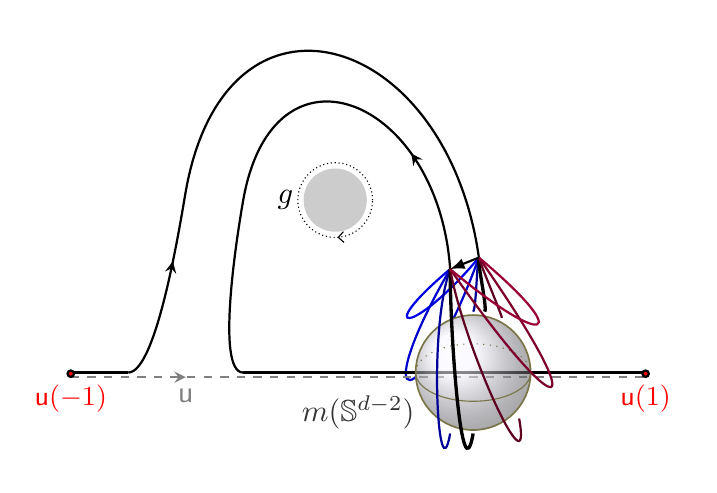
\begin{tikzpicture}[scale=0.73,every node/.style={scale=1.1},even odd rule]
        \clip (0.25,-1.6) rectangle (11.75,6);
        % the leftmost
        \draw[blue!90!black,  thick]
                (7.6,1.8) to[out=-140,in=-130, distance=1.8cm] (8.1,2);
        %the second from left
        \draw[blue!80!black,  thick]
                (7.6,1.8) to[out=-120,in=-110, distance=3cm] (8.1,2);
        \fill[white] (8,0) circle (1cm);
        
        \draw[black, thick] 
            (1,0) -- (2,0)
            (4,0) -- (11,0)
            (6,-0.7) node{\color{black!80!white}$m(\mathbb{S}^{d-2})$};
        \draw[gray,thick, dashed,postaction=decorate,decoration = {markings, mark = at position 0.2 with {\arrow{stealth}}}]
            (1,-0.08) -- (11,-0.08) node[below,pos=0.2]{$\mathsf{u}$};
        % \draw[red, thick]
        %     (8, 0) node[below=1pt]{$x$} circle (1.5pt);

        % sphere
        \foreach \y in {8}{
            \shade[ball color=blue!5!white,opacity=0.55] (\y,0) circle (1cm);
            \draw[black!60!yellow] (\y-1,0) arc (180:360:1cm and 0.5cm);
            \draw[black!60!yellow,dotted] (\y-1,0) arc (180:0:1cm and 0.5cm);
            \draw[black!60!yellow,semithick] (\y,0) circle (1cm);
            }
        % the third from left
        \draw[blue!60!black,  thick]
                        (7.6,1.8) to[out=-110,in=-100, distance=1.15cm] (7.6,-1.06)
                        (8,1.06) to[out=40,in=-120, distance=0.07cm] (8.1,2);
        % middle
        \draw[black, very thick]
                (7.6,1.8) to[out=-90,in=-100, distance=1.15cm] (8,-1.06)
                (8.2,1.06) to[out=40,in=-120, distance=0.07cm] (8.1,2);
        % gp element
        \draw[black,  thick, postaction=decorate,decoration = {markings, mark = at position 0.1 with {\arrow{stealth}} , mark = at position 0.9 with {\arrowreversed{stealth}}}]
                        (2,0) to[out=0,in=-100, distance=0.5cm]
                        (3,3.15) to[out=80,in=98, distance=4cm] (8.1,2)
                        (4,0) to[out=180,in=-100, distance=0.5cm]
                        (4,3) to[out=80,in=94, distance=3cm] (7.6,1.8);
        % the grey hole
        \fill[color=black!20!white] (5.6,3) circle (0.55cm);
        \draw[densely dotted,postaction = decorate,decoration = {markings, mark = at position 0.76 with {\arrowreversed{>}} }] (5.6,3) circle (0.65cm) node[left=0.36cm]{$g$};
        
        % the third from right
        \draw[purple!50!black,  thick]
                (7.6,1.8) to[out=-80,in=-80, distance=1.4cm] (8.8,-0.8)
                (8.5,0.95) to[out=100,in=-80, distance=0.1cm] (8.1,2)
        ;
        % the second from right
        \draw[purple!65!black,  thick]
              (7.6,1.8) to[out=-55,in=-55, distance=3.5cm] (8.1,2);
        % the rightmost
        \draw[purple!80!black,  thick]
                (7.6,1.8) to[out=-40,in=-40, distance=2.2cm] (8.1,2);
        \draw[black, thick,-latex]
                (8.1,2) -- (7.6,1.8);
        % \draw[black,  thick]
        %         % (8.6,2.1) node{\textbf{$\alpha_N$}}
        %         % (10,-1.2) node[purple!60!black]{\textbf{}}
        %         (8.8,4) node{\textbf{$\mathfrak{r}_1(g)=\mathsf{u}_{|,d}=\mathbb{G}_1\circ\mu_{|,d}$}};
        \fill[red,draw=black,thick]
            (1,-0.02) circle (1.6pt) node[below]{\small$\mathsf{u}(-1)$}
            (11,-0.02) circle (1.6pt) node[below]{\small$\mathsf{u}(1)$};
    \end{tikzpicture}
\end{document}